%Przykładowy plik ułatwiający złożenie projektu dyplomowego inżynierskiego.
%UWAGA: Generowany napis na stronie tytułowej o treści PROJEKT DYPLOMOWY INŻYNIERSKI został zaproponowany przeze mnie i nie jest, póki co, potwierdzony przez władze wydziału. Przed ostatecznym oddaniem tak złożonej pracy należy upewnić się jaka powinna być treść tego napisu. W momencie gdy uzyskam informację na temat treści tego napisu, dokonam niezbędnych zmian w źródłach.

\documentclass[eng,printmode]{mgr}
%opcje klasy dokumentu mgr.cls zostały opisane w dołączonej instrukcji

%poniżej deklaracje użycia pakietów, usunąć to co jest niepotrzebne
\usepackage{polski} %przydatne podczas składania dokumentów w j. polskim
%\usepackage[polish]{babel}%alternatywnie do pakietu polski, wybrać jeden z nich
\usepackage[utf8]{inputenc} %kodowanie znakĂłw, zaleĹĽne od systemu
\usepackage[T1]{fontenc} %poprawne składanie polskich czcionek

%pakiety do grafiki
\usepackage{graphicx}
%\usepackage{subfigure}
\usepackage{psfrag}

%pakiety dodające dużo dodatkowych poleceń matematycznych
\usepackage{amsmath}
\usepackage{amsfonts}

%pakiety wspomagające i poprawiające składanie tabel
%\usepackage{supertabular}
\usepackage{array}
\usepackage{tabularx}
\usepackage{hhline}

\usepackage{mathtools}


%pakiet wypisujący na marginesie etykiety równań i rysunków zdefiniowanych przez \label{}, chcąc wygenerować finalną wersję dokumentu wystarczy usunąć poniższą linię
%\usepackage{showlabels}

%definicje własnych poleceń
\newcommand{\R}{I\!\!R} %symbol liczb rzeczywistych, działa tylko w trybie matematycznym
\newtheorem{theorem}{Twierdzenie}[section] %nowe otoczenie do składania twierdzeń

%dane do złożenia strony tytułowej
\title{Detekcja aktywności mówcy w systemach automatycznego rozpoznawania mowy}
\engtitle{Voice activity detection in automatic speech recognition systems}
\author{Paulina Szczerbak}
\supervisor{Prof. dr hab. inż. Ryszard Makowski}
%\guardian{dr hab. inż. Imię Nazwisko Prof. PWr, I-6} %nie używać jeśli opiekun jest tą samą osobą co prowadzący pracę

%\date{2008} %standardowo u dołu strony tytułowej umieszczany jest bieżący rok, to polecenie pozwala wstawić dowolny rok

%poniżej jest lista kierunków i specjalności na wydziale elektroniki, należy wybrać właściwe lub dopisać jeśli nie ma odpowiednich
\field{Automatyka i Robotyka (AIR)}
\specialisation{Technologie informacyjne w systemach automatyki (ART)}

%tutaj zaczyna się właściwa treść dokumentu
\begin{document}
\bibliographystyle{plabbrv} %tylko gdy uĹĽywamy BibTeXa, ustawia polski styl bibliografii

\maketitle %polecenie generujące stronę tytułową
%\dedication{6cm}{Dla mamy i taty heheheheheh xD \texttt{$\backslash$dedykacja}}

\tableofcontents %spis treści

%poniżej znajduje się przykładowa treść dalszej części dokumentu, zainteresowanych zachęcam do rozszyfrowania frazy "Lorem ipsum" :)
\chapter{Wstęp}
Celem niniejszej pracy jest zaprezentowanie wybranych metod detekcji aktywności mówcy (VAD) w systemach automatycznego rozpoznawania mowy w oparciu o napisany program w języku C++. Kolejnym etapem jest porównanie zaimplementowanych metod pod względem dokładności detekcji w separowanych wyrazach oraz w dłuższych ciągach słów.

Rozdział 2. opisuje w uproszczony sposób proces wytwarzania mowy przez człowieka. Prezentuje, w jaki sposób działa aparat mowy oraz z jakich narządów się składa. Na koniec pokazany jest matematyczny model jaki można stworzyć wzorując się na naturalnym systemie generowania mowy.

Rozdział 3. zawiera wyjaśnienie na temat detekcji aktywności mówcy - czym jest oraz gdzie jest wykorzystywana. W tym rodziale opisane są również wybrane algorytmy, które zostały zestawione w dalszej części pracy. Przedstawiona jest zasada ich działania oraz pokrótce wyjaśniona kwestia implementacyjna każdego z nich.
 
Rozdział 4. prezentuje wyniki działania wybranych algorytmów dla separowanych słów. Pokazane są różnice w detekcji oraz ocena każdego z algorytmów.

Rozdział 5. zawiera  wyniki detekcji dla całych ciągów słów oraz porównanie w działaniu wybranych algorytmów i ich ocenę.

\chapter{Generowanie sygnału mowy}
 \section{Mowa w życiu człowieka}
 
 Mowa w życiu większości ludzi stanowi podstawę komunikacji interpersonalnej. Jest sygnałem akustycznym, czyli rozważany jest zakres częstotliwości słyszanych przez człowieka, to jest od 20Hz do 16kHz. Zatem mowa to nic innego jak system artykułowanych dźwięków, które układają się zgodnie z konwencją wybranego języka. Pełni ona funkcję nie tylko komunikacyjną (przekazywanie informacji drugiej osobie o tym, co doświadczyliśmy, czy czego się dowiedzieliśmy), ale również ekspresyjną (można w niej zawrzeć informacje o emocjach nadawcy) oraz regulacyjną (wydawanie i przyjmowanie dyspozycji). 
 
 
 \section{Biologiczny proces generowania mowy}
 Wszelkie metody przetwarzania sygnału mowy muszą bazować na strukturze sygnału, a ta jest niewątpliwie uzależniona od sposobu, w jaki jest on wytwarzany. Niegdyś generowanie sygnałów mowy było domeną jedynie organizmu człowieka, czyli systemu naturalnego. W celu stworzenia systemu, który w jakiś sposób operuje na sygnałach mowy, czyli np. syntezatora mowy, systemu generującego sygnały mowopodobne, systemu automatycznego rozpoznawania mowy czy detekcji aktywności mówcy, należy mieć przynajmniej podstawową wiedzę na temat systemu naturalnego - tego, w jaki sposób działa aparat mowy człowieka.
 
 Wytwarzanie mowy przez człowieka jest procesem niezwykle skomplikowanym, który ma swój początek w mózgu, gdzie następuje konstrukcja wypowiedzi. Później następuje sformułowanie fonetyki i artykulacja poprzez aparat mowy. Ponadto, w procesie generowania mowy można wyróżnić cztery pomniejsze etapy:
	 
	 - proces psychologiczny - wymyślenie i skonstruowanie wypowiedzi,
	 
	 - proces neurologiczny - pobudzenie przez układ nerwowy mięśni, które biorą udział w wytwarzaniu mowy,
	 
	 - proces fizjologiczny - proces kształtowania dźwięków mowy ludzkiej,
	 
	 - proces aerodynamiczny - drgania i przepływ powietrza przez aparat mowy. 
  
  Pierwszym narządem wchodzącym w skład traktu głosowego człowieka są płuca - dostarczają one powietrze do procesu artykulacji, są źródłem zmian ciśnienia akustycznego. Organ mowy człowieka jest napędzany przez wydychane powietrze. Powietrze to, jest prowadzone przez oskrzela i tchawicę do krtani, a drgające w niej struny głosowe modyfikują ciśnienie i wytwarzają dźwięczne fragmenty mowy.  Następnie, dzięki wnękom rezonansowym, tworzonym przez język, podniebienie, zęby oraz wargi, dźwięk ten jest modulowany. Niezwykle ważną rolę przy formowaniu tych wnęk, odgrywają ruchy żuchwy i policzków. Podczas generowania głosek nosowych zamknięta jama ustna spełnia rolę bocznika akustycznego, a dzięki odpowiedniemu ustawieniu języczka podniebienia miękkiego, fala dźwiękowa jest emitowana przez jamę nosową i nozdrza. Struktura traktu głosowego jest przedstawiona schematycznie na rysunku 2.1.

\begin{figure}
	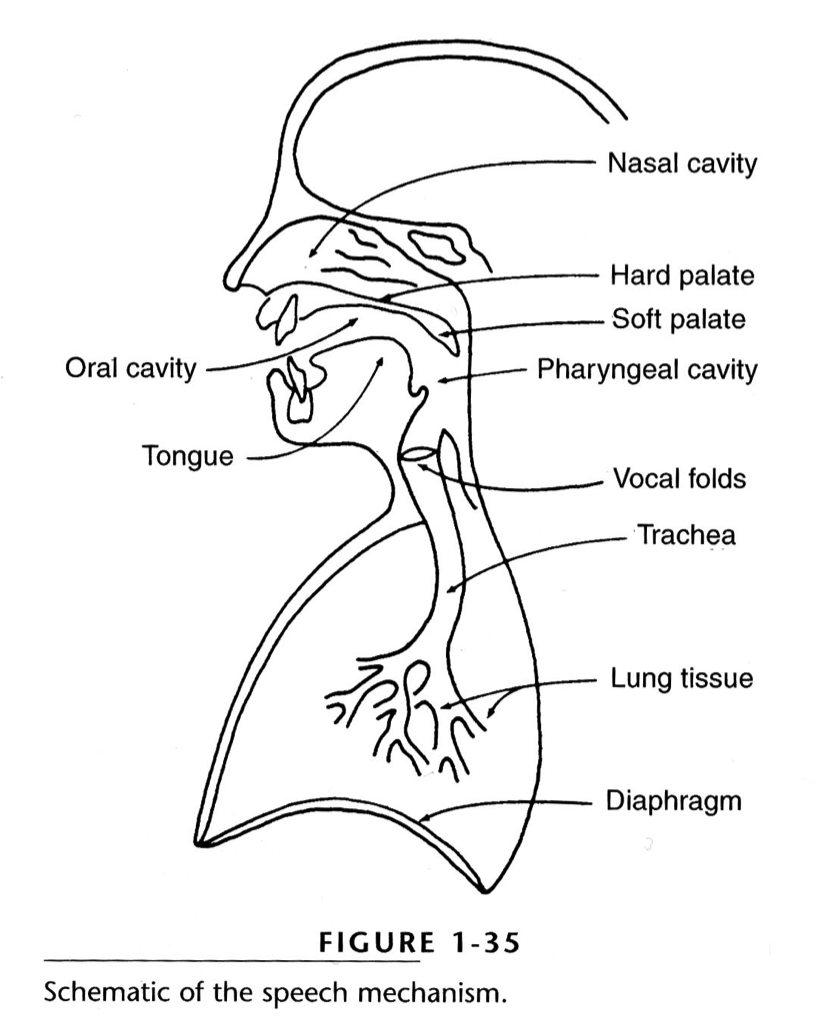
\includegraphics[scale=0.45]{speechmech.png}
	\caption{Aparat mowy człowieka}
\end{figure}

 Ponadto, sterowanie całym systemem generowania mowy jest bardzo złożone i w dużej mierze opiera się na licznych sprzężeniach zwrotnych. Główną rolę odgrywa tutaj sprzężenie zwrotne, które poddaje jakość wydawanych dźwięków bezpośredniej ocenie poprzez analizator słuchowy. Dzięki temu proces artykulacji jest odpowiednio sterowany. Istotę tego sprzężenia zwrotnego potwierdzają trudności z mową wśród ludzi głuchych oraz ludzi słyszących, którzy tymczasowo przebywają w trudnych warunkach środowiskowych, które uniemożliwiają słyszenie własnego głosu.
 
 SCHEMAT Z PDFA STR 23 SPRZERZENIE ZWROTNE  
 
 \section{Matematyczny model procesu generowania mowy}
 \section{Przebieg czasowy i widmo przebiegu}
 //tutaj przykladowy sygnal w dziedzinie czasu i w dziedzinie czestotliwosci 
 
 
  

\chapter{Wybrane metody detekcji aktywności mówcy}
 \section{Czym jest detekcja aktywności mówcy oraz gdzie się ją wykorzystuje}
 + schemat jak w ksiazce RM, w ktorym miejscu jest vad w systemie ARM
 
 Detekcja aktywności mówcy (Voice Activity Detection - VAD) jest powszechnie stosowana w systemach automatycznego rozpoznawania mowy. Podczas rejestrowania wypowiedzi do późniejszego przetwarzania jej przez system ARM, zostaje zarejestrowana cała wypowiedź mówcy, włącznie z częścią, która nie zawiera mowy. Jeżeli we fragmencie jest zawarty sygnał mowy, mówimy, że mówca jest aktywny. Aktywnością mówcy nazywa się emitowny przez niego dźwięk.  Zawartość semantyczna wypowiedzi jest zawarta w głównej mierze we fragmentach, kiedy mówca jest aktywny. Analizowanie całego  zarejestrowanego sygnału mowy, bez wykorzystania systemu VAD, jest oczywiście możliwe, aczkolwiek niepotrzebnie zwiększa czas obliczeń oraz istnieje prawdopodobieństwo, że fragment, gdy mówca nie jest aktywny, zostanie błędnie zaklasyfikowany jako jakiś konkretny fonem - zatem w dużej mierze może popsuć jakość rozpoznania. Detekcja aktywności mówcy w ogólnym przypadku zakłada, że sygnał może występować w dwóch stanach: tylko szum (brak sygnału mowy), szum + sygnał mowy. Korzystając z zagadnienia hipotez ze statystyki, możemy pierwszy stan oznaczyć jako hipotezę $H_{0}$, a drugi jako $H_{1}$, dzięki czemu możemy przedstawić to w następujący sposób:
 \begin{equation}
  \begin{array}{c}
	  H_{0}: f(n)=x(n)\\
	  H_{1}: f(n)=v(n)+x(n)
  \end{array} 	 
 \end{equation}
  Przy takim rozumowaniu konieczne jest określenie statystyki $S(n)$ sygnału, dzięki czemu możliwe będzie dokonywanie detekcji, a w dalszej kolejności zastosowanie kryterium decyzyjnego. Kryterium decyzyjne zwykle polega na porównaniu wartości $S(n)$ z progiem detekcji, który w mniej skomplikowanych algorytmach przyjmuje stałą wartość. Natomiast w tych bardziej złożonych, może występować np. jako funkcja czasu. Wartość stałej wartości progu jest ustalana w wyniku teoretycznych rozważań lub empirycznie. Zatem detekcja $\gamma(n)$, w ogólnej postaci, będzie prezentować się następująco:
   \begin{equation}
   \begin{array}{c}
	   S(n)\geq\gamma(n)\to H_{1}\\
	   S(n)<\gamma(n)\to H_{0}
   \end{array} 	 
   \end{equation}
 
	 
 \section{Algorytm bazujący na energii pojedynczej ramki}
 \subsection{Próg detekcji}
 $//TODO:******************************************************************************$
 Zakłada się, że przed każdą wypowiedzią każdy człowiek potrzebuje chwili na nabranie powietrza, mlaśnięcie czy aktywację strun głosowych. W związku z tym, zwykle pierwsze 200ms w nagraniu to stan ciszy. Początkowy próg detekcji jest więc ustalany jako średnia energia z pierwszych 100ms nagrania.
 \subsection{Zasada działania algorytmu}
 Jest to  najprostszy z przedstawionych algorytmów. Dzięki temu ma również najniższa złożoność obliczeniową, jednak kosztem jest jego niższa dokładność. Bazuje ona na policzeniu energii dla kolejnych ramek sygnału, zgodnie ze wzorem:
 
$ Em = Sum(n=0, l, x^2(n))$
		gdzie: m - numer ramki
				l - długość ramki.
				
		Następnie wartości poszczegolnych ramek porównywane są z ustalonym wcześniej progem detekcji - jeżeli przekraczają jego wartość, to uznaje się, że zawierają mowę, a jeżeli nie, to w ramce mowy nie ma. Zwykle długość ramki przyjmuje się z przedziału 20-30ms, w tej pracy przyjęto, że l = 30ms. 
		

 \section{Algorytm SFF (Single Frequency Filtering)} 
 \subsection{Zasada działania algorytmu}
 Algorytm Single Frequency Filtering to metoda działająca w oparciu o obwiednię sygnału podzielonego na pasma z filtracją pojedynczych częstotliwości. Do dokonania detekcji, należy wcześniej policzyć obwiednię dla sygnału podzielonego na 185 pasm - od 30Hz do 4000Hz, co 20Hz. Wybrany przedział częstotliwości pokrywa się z użytecznym pasmem, który jest wykorzystywany przez mowę. Poniżej zostały przedstawione kolejne kroki potrzebne do policzenia 185 obwiedni i odpowiedniego przekształcenia ich w funkcję czasu, na której będzie można dokonać detekcji.
 
 \subsubsection{1. Obwiednie sygnału dla każdej częstotliwości}
 Sygnał mowy w zdyskretyzowanej dziedzinie czasu $s(n)$ jest różniczkowany i jest rozumiany jako $x(n) = s(n) - s(n-1)$. Częstotliwość próbkowania to $fs$. Sygnał $x(n)$ jest przemnażany przez zespoloną sinusoidę o danej znormalizowanej częstotliwości śr omega k. Wynikowa operacja w dziedzinie czasu jest dana jako: $\bar{\omega}_{k}$. Wynik tej operacji w dziedzinie czasu jest dany jako: 
 
 $$x_{k}(n) = x(n)e^{j\bar{\omega}_{k}n}$$,
 
 gdzie $$\bar{\omega}_{k} = \frac{2\pi\bar{f_{k}}}{f_{s}}$$
 
 Kiedy pomnożymy $x(n)$ przez $e^{j\bar{\omega}_{k}n}$, wynikowe widmo $x_{k}(n)$ będzie przesuniętym widmem x(n). Czyli:
 
 $$X_{k}(\omega) = X(\omega - \bar{\omega}_{k})$$,
 
 gdzie $X_{k}(\omega)$ i $X(\omega)$ to odpowiednio widma  $x_{k}(n)$ i $x(n)$.
 
 Sygnał $x_{k}(n)$ jest przepuszczany przez jednobiegunowy filtr, którego transmitancja jest dana jako:
 
 $$H(z) = \frac{1}{1+rz^{-1}}$$
 
 Jednobiegunowy filtr ma biegun na osi liczb rzeczywistych w odległości $r$ od początku układu współrzędnych. Lokalizacja pierwiastka jest w $z = -r$ na płaszczyśnie liczb zespolonych, co odpowiada połowie częstotliwości próbkowania, np $fs/2$. Wyjście filtra $y_{k}(n)$ jest dane jako:
 
 $$y_{k}(n) = -r y_{k}(n-1)+x_{k}(n)$$
 
  Obwiednia sygnału yk(n) jest dana jako:
  
  $$e_{k}(n) = \sqrt{y_{kr}^2(n) + y_{ki}^2(n)}$$ 			(10), 
  
  gdzie $y_kr(n)$ i $y_{ki}(n)$ są odpowiednio częścią rzeczywista i urojoną $y_{k}(n)$.
  
  Kiedy filtrowanie $x_{k}(n)$ będzie zrobione dla $\frac{f_{s}}{2}$, powyższa obwiednia $e_{k}(n)$ będzie odpowiadać obwiedni sygnału $x_{k}(n)$ przefiltrowanego w pożądanej częstotliwości
  
  $$f_{k} = \frac{f_{s}}{2} - \bar{f_{k}}$$.
  
  Powyższa metoda estymowania obwiedni składowej dla częstotliwości $f_{k}$ jest określana jako podejście filtracji pojedynczych częstotliwości (Single Frequency Filtering). Wybór filtra z biegunem w $z=-r$ do estymacji obwiedni przefiltrownego sygnału wydaje się być bardziej odpowiedni, jako że obwiednie są obliczane w możliwie najwyższych częstotliwościach $(f_{s}/2)$. Ponadto, wybór filtru w stałej częstotliwości dla jakiejkolwiek pożądaniej częstotliwości $f_{k}$ zapobiega efektu przeskalowania w związku z różnymi wzmocnieniami filtrów w różnych częstotliwościach. Jeżeli biegun zostanie wybrany z obszaru na kole jednostkowym, np $z=r=-1$, może to skutkować niestabilnością wyjścia filtru. Stabilność filtru jest zapewniona dzięki przesunięciu bieguna nieco bardziej wewnątrz koła jednostkowego. Z tego powodu $r$ zostało dobrane jako 0.99.
  
  W tym badaniu obwiednia została obliczona dla każdych 20Hz w przedziale od 300Hz do 3000Hz jako funkcja w dziedzinie czasu. Wybrany został przedział częstotliwości 300-4000Hz, ponieważ pokrywa się z użytecznym pasmem wykorzystywanym przez mowę. Zatem mamy obwiednie dla 185 częstotliwości jako funkcja w dziedzinie czasu. Zasadniczo obwiednia może zostać obliczona dla każdej pożądanej częstotliwości.
  
  \subsubsection{2. Ważone składowe obwiedni sygnału mowy}
  Kiedy sygnał mowy ma bardzo dużą rozpiętość tonalną w dziedzinie częstotliwości, sygnał może mieć wysoką wartość mocy w niektórych częstotliwościach w każdej chwili czasowej. W tych częstotliwościach SNR będzie miał większą wartość, jako, że moc szumu będzie prawdopodobnie mniejsza w związku z większym rozkładem jednostajnym mocy. Nawet dla szumów z nierównomiernym rozkładem mocy, niższe korelacje próbek szumu skutkują w niższej rozpiętości tonalnej w rozpiętości mocy szumu przez częstotliwość, w porównaniu z sygnałem mowy. Zauważmy, że widmowa rozpiętość tonalna daje przejaw korelacji próbek w dziedzinie czasu. 
  
  Moc szumu tworzy funkcję cechy (podłogi) dla obwiedni dla każdej częstotliwości i poziom cechy zależy od rozkładu mocy szumu wobec częstotliwości. Podłoga jest bardziej jednorodna wobec czasu, jeżeli szum jest niemalże stacjonarny. Nawet jeżeli szum jest niestacjonarny, jest względnie stacjonarny ponad większymi przerwami w czasie niż sygnał mowy. W takich przypadkach, poziom cechy może zostać obliczony ponad długimi przerwami w dziedzinie czasu dla każdej częstotliwości, jeżeli jest to potrzebne.
  
  Żeby zrekompensować efekt szumu, wartość wagi dla każdej częstotliwości jest obliczana używając wartości funkcji cechy. Dla każdego wyrażenia, średnia $(\mu_{k})$ z 20 \% najmniejszych wartości, wartości obwiedni dla każdej częstotliwości $f_{k}$ jest wykorzystywana do obliczenia znormalizowanej wagi wartości $\omega_{k}$ dla danej częstotliwości. Wybór akurat 20\% wartości jest oparty o założenie, że w jest przynajmniej 20\% ciszy w każdym wyrażeniu mowy. Znormalizowana waga wartości w każdej częstotiwości jest dana jako:
  
  
  $$\omega_{k} = \frac{\frac{1}{\mu_{k}}}{\sum_{l=1}^{N}	\frac{1}{\mu_{t}}},$$
  
  gdzie N to liczba kanałów.
  
  Obwiednia $e_{k}(n)$ dla każdej częstotliwości $f_{k}$ jest przemnażana przez wartość wagi $w_{k}$ w celu zrekompensowania poziomu szumu w tej częstotiwości. Wynikowa obwiednia jest określana jako obwiednia z ważonymi komponentami. Zauważmy, że przez to ważenie, obwiednia dla każdej częstotliwości jest dzielona przez estymatę cechy szumu $u_{k}$. 
  *****************************************************************!!Rys. 1 pokazuje obwiednie i odpowiadające ważone obwiednie dla różnych częstotliwości w sygnale mowy  zaszumionym szumem różowym z 10dB SNR w porównaniu z obwiedniami dla sygnału niezaszumionego. Można zaobserwować, że cechy mowy są lepiej wyeksponowane w ważonych obwiedniach (rys 1(d)), ponieważ wagi redukują efekt szumu. Do porównania, obwiednie zostały przeskalowane do tej samej wartości. 
  
  Do wszystkich sygnałów została dodana mała ilośc białego szumu (100dB SNR), żeby mieć pewność, że wartość funkcji cechy nie jest zerem. Dla obliczeń wk, wartości w dodanych obszarach ciszy nie będą rozważane. 
  
  W każdej chwili czasu średnia ($\mu(n)$) kwadratu ważonych obwiedni obliczonych  wobec częstotliwości odpowiada w przybliżeniu energii sygnału w danej chwili (rys 2(c)) Oczekuje się, że $\mu(n)$ będzie wyższe dla mowy, niż dla szumu w obszarach, gdzie występuje sygnał mowy, ponieważ wartosci szumu są o obniżonej wadze. W każdej chwili czasu, odchylenie standardowe ($\sigma(n)$) kwadratu ważonych obwiedni rownież będzie względnie wyższe dla mowy niż dla szumu w obszarach mowy - związane jest to ze strukturą formantu. Dlatego $\sigma(n)+ \mu(n)$ jest na ogół wyższe w obszarach mowy i niższe w regionach pozbawionych mowy. Ponieważ oczekuje się, że rozpiętość szumu (po kompensacji) będzie niższa, zaobserwowano, że wartości $\sigma(n)-\mu(n)$ są zwykle niższe w obszarach pozbawionych mowy, w porównaniu do obszarów zawierających mowę (rys. 2(e)). Pomnożenie (sigma(n) + u(n)) przez (sigma(n)+ u(n)) daje $(sigma^2(n) - u^2(n))$, co podkreśla kontrast pomiędzy obszarami zawierającymi mowę i tymi, które mowy nie zawierają. *********************************************************************Rys 2 i 3 przedstawia cechy u(n), sigma(n) oraz (sigma(n)-u(n)) dla wyrażenia zdegradowanego szumem różowym o odpowiednio SNR=-10dB i SNR=5dB.   
  
  W związku z dużą rozpiętością tonalną wartości $(sigma^2(n) - u^2(n))$, ciężko jest zaobserwować obszary mowy z małymi wartościami  $(sigma^2(n) - u^2(n))$. Aby podkreślić kontrast pomiędzy obszarami mowy i obszarami niezawierającymi mowy, rozpiętość tonalna jest redukowana poprzez obliczenie
  
   $$\delta(n) =\sqrt[M]{|{(\sigma^2(n) - \mu^2(n))}|},$$ gdzie M zostało wybrane jako 64
   
    Wartość M nie jest decydująca. Każda wartość M z przedziału 32-256 wydaje się być dobra, aby zapewnić dobry kontrast pomiędzy obszarami zawierającymi mowę, a tymi, które mowy nie zawierają na wykresie $\delta(n)$. W obliczeniach $\delta(n)$ brana jest po uwagę tylko wartość bezwzględna wartości chwilowej $(\sigma^2(n) - \mu^2(n))$. Jeżeli znak wyrażenia $(\sigma^2(n) - \mu^2(n))$. jest przypisany(?) do delta(n), wartości będą wahać się w okolicach zera w obszarach pozbawionych mowy dla większości typów szumów (zobacz ************************rys 2(f) dla szumu różowego), ale krótki czas (20-40msec) tymczasowych średnich wartości będzie mały i będzie się wahał, sprawiając, że cecha szumu będzie nierówna. To powoduje trudności w ustaleniu progu detekcji dla obszarów pozbawionych mowy. Wartości $\delta(n)$ będą miały wysoką średnią w obszarach pozbawionych mowy z małą średnią wariancją (*********rys 2(g)). Pomoże to w ustaleniu odpowiedniego progu do odizolowania obszarów pozbawionych mowy od tych, które mowę zawierają. Zakres $\delta(n)$ ze znakiem (**********************rys. 2(f)) jest inny niż wartości $\delta(n)$ (***********************rys. 2(g)). Mały tymczasowy obszar wartości $\delta(n)$ w obszarach niezawierających  mowy i jego średnia wartość pomagają w dobraniu pasującego progu. Wartości $\delta(n)$ w obszarach niezawierających mowy są podyktowane poziomem szumu. Wartości $\delta(n)$ w obszarach niezawierających mowy są wyższe dla sygnału zaszumionego szumem różowym -10dB SNR (*************rys 2(g)) niż dla 5dB SNR (**************rys 3(g)). Zauważmy, że rozważając wartości  $\delta(n)$ bez znaku, tracimy trochę zalet w rozróżnialności obszarów niezawierających mowy, które maja zarówno dodatnie, jak i ujemne wartości - natomiast obszary zawierające mowę mają w większości dodatnie wartości. Wartości $\delta(n)$ z $M=64$ są wykorzystywane do dalszego przetwarzania do podejmowania decyzji. Warto zauważyć zmiany w przeskalowaniu na rys 2(f) i 2(g) oraz 3(f) i 3(g), aby zrozumieć istotę używania wartości bezwzględnej, np $\delta(n)$ bez znaku.
    
  \subsubsection{3. Logika podejmowania decyzji}
  
  \subsection{Próg detekcji}

 
\section{Zmieniony algorytm Single Frequency Filtering}
\chapter{Implementacja programu}
Do zaimplementowania algorytmów skorzystano z biblioteki Aquila, która wspiera operacje na sygnałach oraz z standardowych bibliotek C++, takich jak cmath, stl.



\chapter{Wyniki dla pojedynczych słów}
 \section{Sposób oceny}
	Do przeprowadzenia badań zostało wybranych 5 sygnałów zawierających ciągi słów. Pierwszy etap badań założył manualne wybranie próbek zawierających początki oraz końce wypowiedzi, rozważone zostały dwa przypadki, gdy: 
	1.  mowa rozpoczyna się w momencie nabrania powietrza przez mówcę i aktywację strun głosowych,
	2. 	mowa rozpoczyna się w momencie generowania słyszalnych dźwięków przez mówcę.
	Następnie te same sygnały zostały zbadane przez 3 algorytmy detekcji, które również wybrały numery próbek, które miały reprezentować początki i końce mowy. Dla każdego pomiaru wykonano 10 prób i ostateczne wartości poddane badaniom są średnią wartością z tych prób. 
	
	 Następnie została policzona wartość bezwzględna próbki wybranej manualnie oraz próbki wybranej przez algorytm. Wyniki dla poszczególnych algorytmów, w dwóch rozważanych przypadkach zostały przedstawione w tabeli poniżej.
 \section{Wyniki}

\chapter{Wyniki dla ciągów słów}

\chapter{Podsumowanie}

\addcontentsline{toc}{chapter}{Bibliografia} %utworzenie w spisie treści pozycji Bibliografia
\bibliography{bibliografia} % wstawia bibliografię korzystając z pliku bibliografia.bib - dotyczy BibTeXa, jeżeli nie korzystamy z BibTeXa należy użyć otoczenia thebibliography
%biologiczny proces
%http://otworzksiazke.pl/images/ksiazki/sygnal_mowy/sygnal_mowy.pdf
%
%http://www.iaeng.org/IJCS/issues_v36/issue_4/IJCS_36_4_16.pdf


%opcjonalnie może się tu pojawić spis rysunków i tabel
 \listoffigures
 \listoftables
\end{document}

